\documentclass[12pt]{article}

\usepackage[utf8]{inputenc}
\usepackage{latexsym,amsfonts,amssymb,amsthm,amsmath,mathrsfs,mathtools}
\usepackage[makeroom]{cancel}
\usepackage {tikz}
\usepackage{hyperref}
\usetikzlibrary {positioning}
\usepackage{fdsymbol}

\usepackage[ruled,vlined]{algorithm2e}

\setlength{\parindent}{0in}
\setlength{\oddsidemargin}{0in}
\setlength{\textwidth}{6.5in}
\setlength{\textheight}{8.8in}
\setlength{\topmargin}{-0.7in}
\setlength{\headheight}{18pt}

\newcommand*{\union}{\cup}
\newcommand*{\inter}{\cap}

\DeclarePairedDelimiter\floor{\lfloor}{\rfloor}
\DeclarePairedDelimiter\ceil{\lceil}{\rceil}

\definecolor {processblue}{cmyk}{0.96,0,0,0}

\makeatletter

\makeatother

\title{Topics in Algorithms - Assignment 2}
\author{Kishlaya Jaiswal}

\begin{document}

\maketitle

Following are the exercises from \href{http://math.mit.edu/~goemans/18453S17/matching-nonbip-notes.pdf}{http://math.mit.edu/~goemans/18453S17/matching-nonbip-notes.pdf}

\subsection*{Exercise 2.1}

Consider the following graph:
\begin{center}
\begin{tikzpicture}[shorten >=1pt,->]
  \tikzstyle{vertex}=[circle ,top color =white , bottom color = processblue!20 ,
draw,processblue , text=blue , minimum width =1 cm]
  \node[vertex] (G_1) at (9,0)  {1};
  \node[vertex] (G_2) at (6,0)  {2};
  \node[vertex] (G_3) at (3,0) {3};
  \node[vertex] (G_4) at (0.927,2.853)   {4};
  \node[vertex] (G_5) at (-2.427,1.763)  {5};
  \node[vertex] (G_6) at (-2.427,-1.763)  {6};
  \node[vertex] (G_7) at (0.927,-2.853)  {7};
  \node[vertex] (G_8) at (0.927,5.853)   {8};
  \node[vertex] (G_9) at (-5.427,1.763)  {9};
  \node[vertex] (G_10) at (-5.427,-1.763)  {10};
  \node[vertex] (G_11) at (0.927,-5.853)  {11};

  \draw (G_1) -- (G_2) -- cycle;
  \draw[ultra thick, red] (G_2) -- (G_3) -- cycle;
  \draw (G_3) -- (G_4) -- cycle;
  \draw[ultra thick, red] (G_4) -- (G_5) -- cycle;
  \draw (G_5) -- (G_6) -- cycle;
  \draw[ultra thick, red] (G_6) -- (G_7) -- cycle;
  \draw (G_7) -- (G_3) -- cycle;
  \draw (G_4) -- (G_8) -- cycle;
  \draw (G_5) -- (G_9) -- cycle;
  \draw (G_6) -- (G_10) -- cycle;
  \draw (G_7) -- (G_11) -- cycle;
\end{tikzpicture}
\end{center}

When we shrink the blossom, we would get
\begin{center}
\begin{tikzpicture}[shorten >=1pt,->]
  \tikzstyle{vertex}=[circle ,top color =white , bottom color = processblue!20 ,
draw,processblue , text=blue , minimum width =1 cm]
  \node[vertex] (G_1) at (6,0)  {1};
  \node[vertex] (G_2) at (3,0)  {2};
  \node[vertex] (G_3) at (0,0) {3};
  \node[vertex] (G_8) at (0,3)   {8};
  \node[vertex] (G_9) at (-3.427,1.763)  {9};
  \node[vertex] (G_10) at (-3.427,-1.763)  {10};
  \node[vertex] (G_11) at (0,-3)  {11};

  \draw (G_1) -- (G_2) -- cycle;
  \draw[ultra thick, red] (G_2) -- (G_3) -- cycle;
  \draw (G_3) -- (G_8) -- cycle;
  \draw (G_3) -- (G_9) -- cycle;
  \draw (G_3) -- (G_10) -- cycle;
  \draw (G_3) -- (G_11) -- cycle;
\end{tikzpicture}
\end{center}

An augmenting path in the graph $G/B$ is: $1 \rightarrow 2 \rightarrow 3 \rightarrow 11$, which gives the following maximum matching $M^*/B$ in $G/B$

\begin{center}
\begin{tikzpicture}[shorten >=1pt,->]
  \tikzstyle{vertex}=[circle ,top color =white , bottom color = processblue!20 ,
draw,processblue , text=blue , minimum width =1 cm]
  \node[vertex] (G_1) at (6,0)  {1};
  \node[vertex] (G_2) at (3,0)  {2};
  \node[vertex] (G_3) at (0,0) {3};
  \node[vertex] (G_8) at (0,3)   {8};
  \node[vertex] (G_9) at (-3.427,1.763)  {9};
  \node[vertex] (G_10) at (-3.427,-1.763)  {10};
  \node[vertex] (G_11) at (0,-3)  {11};

  \draw[ultra thick, red] (G_1) -- (G_2) -- cycle;
  \draw (G_2) -- (G_3) -- cycle;
  \draw (G_3) -- (G_8) -- cycle;
  \draw (G_3) -- (G_9) -- cycle;
  \draw (G_3) -- (G_10) -- cycle;
  \draw[ultra thick, red] (G_3) -- (G_11) -- cycle;
\end{tikzpicture}
\end{center}

But this leads to the augmenting path $1 \rightarrow 2 \rightarrow 3 \rightarrow 4 \rightarrow 5 \rightarrow 6 \rightarrow 7 \rightarrow 11$ in $G$ and gives the following matching $M^*$ (which is not a maximum matching):

\begin{center}
\begin{tikzpicture}[shorten >=1pt,->]
  \tikzstyle{vertex}=[circle ,top color =white , bottom color = processblue!20 ,
draw,processblue , text=blue , minimum width =1 cm]
  \node[vertex] (G_1) at (9,0)  {1};
  \node[vertex] (G_2) at (6,0)  {2};
  \node[vertex] (G_3) at (3,0) {3};
  \node[vertex] (G_4) at (0.927,2.853)   {4};
  \node[vertex] (G_5) at (-2.427,1.763)  {5};
  \node[vertex] (G_6) at (-2.427,-1.763)  {6};
  \node[vertex] (G_7) at (0.927,-2.853)  {7};
  \node[vertex] (G_8) at (0.927,5.853)   {8};
  \node[vertex] (G_9) at (-5.427,1.763)  {9};
  \node[vertex] (G_10) at (-5.427,-1.763)  {10};
  \node[vertex] (G_11) at (0.927,-5.853)  {11};

  \draw[ultra thick, red] (G_1) -- (G_2) -- cycle;
  \draw (G_2) -- (G_3) -- cycle;
  \draw[ultra thick, red] (G_3) -- (G_4) -- cycle;
  \draw (G_4) -- (G_5) -- cycle;
  \draw[ultra thick, red] (G_5) -- (G_6) -- cycle;
  \draw (G_6) -- (G_7) -- cycle;
  \draw (G_7) -- (G_3) -- cycle;
  \draw (G_4) -- (G_8) -- cycle;
  \draw (G_5) -- (G_9) -- cycle;
  \draw (G_6) -- (G_10) -- cycle;
  \draw[ultra thick, red] (G_7) -- (G_11) -- cycle;
\end{tikzpicture}
\end{center}

This does not contradict theorem $2.2$ because if $M^*$ were to be a maximum matching in $G$, then the theorem says: \textsl{Let $B$ be a blossom with respect to $M^*$ . Then $M^*$ is a maximum size matching in $G$ if and only if $M^*/B$ is a maximum size matching in $G/B$}. Notice that $B$ was a blossom with respect to initial matching $M$ and not $M^*$ and hence the hypothesis of the theorem is not satisfied.

\subsection*{Exercise 2.2}

Recall \textbf{Berge's lemma}: a matching $M$ in a graph $G$ is maximum if and only if there is no augmenting path wrt $M$ in $G$.

Further note that if a matching matches the vertices in $S$, then augmenting this matching along any augmenting path will still keep the vertices in $S$ matched.

Therefore, suppose a matching $M$ covers $S$; if $M$ is already maximum then we are done. Otherwise, by Berge's lemma there is an augmenting path wrt to $M$. Augment along this path to get a new matching $M'$. Then $|M'| > |M|$ and $M'$ also covers $S$. Thus, repeating this $O(|V|)$ times, we get a maximum matching $M^*$ which covers $S$.

\subsection*{Exercise 2.3}

\subsubsection*{(a)}
By Tutte's theorem, given any maximum matching $M$, we have
$$|M| = |U| + \sum_{i=1}^k \floor*{\frac{|K_i|}{2}} = \frac{1}{2}\left(|V| + |U| - o(G \setminus U)\right) (\spadesuit)$$

And after removing $U$, any maximum matching can $M$ can use atmost $k_i = \floor*{\frac{|K_i|}{2}}$ many edges from $K_i$, therefore it is certain that $M$ uses atmost $k_i$ edges from $G[K_i]$. If it uses strictly less than $k_i$ edges from $G[K_i]$ then note that size of $M$ is also strictly less than $|U| + \sum_{i=1}^k \floor*{\frac{|K_i|}{2}}$ which is a contradiction to $(\spadesuit)$.

Hence the vertices in $G[K_i]$ with even $|K_i|$ are perfectly matched whereas with odd $|K_i|$ are perfectly matched except for one vertex.

\subsubsection*{(b)}
First, suppose some vertex in $u \in U$ remains unmatched in $M$. Then even if we remove this vertex $u$ from the graph, the number of odd components after removing $U \setminus \{u\}$ remains unchanged, so for the new graph thus obtained, we have the following inequality:
$$|M| \leq \frac{1}{2}((|V|-1) + (|U|-1) - o(G \setminus U)) = \frac{1}{2}(|V| + |U| - o(G \setminus U)) - 1$$
which is again a contradiction to $(\spadesuit)$.

Now suppose that $u$ is matched to a vertex in $v \in U$. Then if we remove the vertices $\{u,v\}$ from the graph, then the number of odd components after removing $U \setminus \{u,v\}$ remains unchanged and also the size of $M$ decreases by $1$, so for the new graph thus obtained, we have the following inequality:
$$|M|-1 \leq \frac{1}{2}((|V|-2) + (|U|-2) - o(G \setminus U)) = \frac{1}{2}(|V| + |U| - o(G \setminus U)) - 2$$
which is again a contradiction to $(\spadesuit)$.

Thus, each vertex $u \in U$ is matched to a vertex not in $U$ but since all the vertices in even components are matched among themselves, the only possibility is that $u$ is matched to a vertex in some odd component $K_i$.

\subsubsection*{(c)}
From the above two results, we get that
\begin{itemize}
    \item Every vertex in $U$ is matched
    \item Every vertex in an even component $K_i$ is matched
\end{itemize}
Therefore, if some $v \in V$ is unmatched, then it has to belong to some odd component $K_i$.

\subsection*{Exercise 2.4}

Yes there could be several minimizers in the Tutte Berge formula. A simple example is that of two vertices joined by a single edge, in which case maximum matching is of size $1$ and we could choose $U$ to be either of the vertices to get $1 = \frac{1}{2}(2 + 1 - 1)$.

Another example with different sizes of $U$: Both $U=\phi$ and $U = \{v\}$ give $2 = \frac{1}{2}(5 + 0 - 1) = \frac{1}{2}(5 + 1 - 2)$ in the given graph below:

\begin{center}
\begin{tikzpicture}[shorten >=1pt,->]
  \tikzstyle{vertex}=[circle ,top color =white , bottom color = processblue!20 ,
draw,processblue , text=blue , minimum width =1 cm]
  \node[vertex] (G_1) at (8,0) {};
  \node[vertex] (G_2) at (5,0)  {v};
  \node[vertex] (G_3) at (2,0) {};
  \node[vertex] (G_4) at (-0.8,1.5) {};
  \node[vertex] (G_5) at (-0.8,-1.5) {};

  \draw (G_1) -- (G_2) -- cycle;
  \draw (G_2) -- (G_3) -- cycle;
  \draw (G_3) -- (G_4) -- cycle;
  \draw (G_4) -- (G_5) -- cycle;
  \draw (G_5) -- (G_3) -- cycle;
\end{tikzpicture}
\end{center}


\subsection*{Exercise 2.5}

For a graph $G$ and $S \subseteq V(G)$, define \textsl{deficiency of S} $def(S) = o(G \setminus S) - |S|$. And $def(G) = \max_{S \subseteq V} def(S)$.

Therefore, Tutte-Berge formula now translates to: for any maximum matching $M$, $|M| = \frac{1}{2}(|V| - def(G))$
\newline

\textbf{Parity Lemma} Let $|V| = n$ and $S \subseteq V$, then $def(S) \equiv n (\mod 2)$
\begin{proof}
Counting vertices in $S$ and the components in $G \setminus S$, we have $|S| + o(G \setminus S) \equiv n (\mod 2)$.
\end{proof}

\textbf{Lemma 2} Let $T$ be a maximal set of maximum deficiency in a graph $G$. Then every component of $G \setminus T$ is odd and factor-critical.
\begin{proof}
Let $C$ be any component of $G \setminus T$ and $u \in C$, then $\forall S \subseteq C-u$, we have
\begin{align*}
    def_G(T \union u \union S) &= o(G-T-u-S) - (|T|+1+|S|) \\
    &= (o(G \setminus T) - 1 + o(C-u-S)) - (|T|+1+|S|) \\
    &= o(G \setminus T) - |T| + o(C-u-S) - |S| - 2 \\
    &= def_G(T) + def_{C-u}(S) - 2 \\
    \implies def_{C-u}(S) &= def_G(T \union u \union S) - def_G(T) + 2
\end{align*}
By our choice of $T$, $def_G(T \union u \union S) < def_G(T)$ and by Parity lemma, $def_G(T \union u \union S)$ and $def_G(T)$ have same parity. Thus $def_{C-u}(S) \leq 0$, $\forall S \subseteq C-u$ and hence $C-u$ has a perfect matching (Tutte's theorem) and so $C$ is critical. It follows that $C$ is of odd-size.

(Alternatively, if $C$ is a component of even size, then adding to $T$ any leaf of a spanning tree of $C$ creates a larger set with the same deficiency as $T$ which contradicts the choice of $T$. And hence all components are odd).
\end{proof}

Next for any $T \subseteq V$, we define auxillary bipartite graph $H(T)$ by contracting each component of $G \setminus T$ to a single vertex and deleting edges within $T$. Let $U$ denote the set of contracted vertices of components then $H(T)$ is a $(T,U)$ bipartite graph with an edge $t-u$ for $t \in T, u \in U$ iff $t$ has a neighbour in G in the component of $G \setminus T$ corresponding to $u$.
\newline

\textbf{Lemma 3} If $T$ is a maximal set of maximum deficiency in a graph $G$. then $H(T)$ contains a matching that covers $T$.

\begin{proof}
For $S \subseteq T$ , all vertices of $U - N_{H(T)}(S)$ are odd components of $G \setminus (T \setminus S)$. By the choice of $T$ , we have $(|U|-|N_{H}(S)|) - |T \setminus S| \leq def(T \setminus S) \leq def(T)$. Since $def(T) = |U| - |T|$,
the inequality simplifies to $|S| \leq |N_H(S)|$. Thus Hall’s Condition holds, and $H(T)$ has a matching that covers $T$.
\end{proof}

Now let $T$ be a maximal set of deficiency $def(G)$. If we show that $def(C) = def(T)$, then for any maximum matching $M$:
$$|M| = \frac{1}{2}(n-def(G)) = \frac{1}{2}(n-def(C)) = \frac{1}{2}(|V|+|C|-o(G \setminus C))$$
and hence $C$ is a minimizer in the Tutte-Berge formula.

We begin by noting that $T$ is a minimizer of the Tutte-Berge formula and so $2|M| = n - def(G)$ implies that exactly $def(G)$ vertices are not covered by $M$. Furthermore. we have proved in exercise $2.3$ that $M$ matches each vertex of $T$ with a distinct component of $G \setminus T$ (which are all odd - lemma 2) and also since $M$ is maximum and each of these components is factor-critical (lemma 2), $M$ matches each of these components near-perfectly.

Now consider the bipartite-graph $H(T)$. By lemma 3, there is a $T$-saturating matching and therefore Hall's theorem says $|N_{H(T)}(S)| \geq |S|$, $\forall S \subseteq T$. Because $|N_{H(T)}(\phi)| = |\phi|$, we consider a maximal subset $R$ for which the equality is achieved in Hall's condition, so $|N_{H(T)}(R)| = |R|$. Let $R'$ be the union of all vertices of the components of $N_{H(T)}(R)$.
\newline

\begin{figure}[htp]
    \centering
    \includegraphics[width=12cm]{gallai.jpg}
    \caption{Gallai Decomposition}
    \label{fig:gallai}
\end{figure}

\textbf{Claim} $D = R \union R'$, $C = T \setminus R$ and $B = V \setminus (T \union R')$.
\begin{proof}
We observe that $D$ is defined to be the set of \textsl{essential} vertices which doesn't have any neighbours in \textsl{inessential} vertices. We show that the same property holds for $R \union R'$ as well. Since every maximum matching $M$ matches $T$, and hence $R$, we conclude that $R$ is a subset of essential vertices and so is $R'$ as any maximum matching matches $R$ to distinct components of $G[R']$. Furthermore, both $R$ and $R'$ don't have neighbour in other components of $G \setminus T$, that is $R \union R'$ doesn't have a neighbours in \textsl{inessential} vertices (as $T$ only consists of essential vertices). Therefore, $D = R \union R'$.

Let $H' = H(T) - (R \union N_{H(T)}(R))$. For any $S \subset T \setminus R$, we have $|N_{H(T)}(S)| > |S|$ (because if there was equality for some set, then we could have added it to $R$ thereby contradicting its maximality). This means even if we delete a vertex $v$ from $N_{H'}(T \setminus R)$, Hall's condition still holds and so it has a $T \setminus R$ saturating matching, which omits $v$. This tells us all vertices of $V \setminus (T \union R')$ are inessential. This can be seen as follows: fix a vertex $x \in V \setminus (T \union R')$. Let $C$ be the component to which it belongs. By lemma 2, $C$ is factor-critical. So if we delete $x$, then we can find a perfect matching in $C - x$. So we delete this component $C$ and note that it corresponds to deleting a vertex $v \in N_{H'}(T \setminus R)$ which has a maximum matching already.

Therefore, we get that $V \setminus (T \union R') \subseteq B$ but note that $T$ only consists of essential vertices. And so $B = V \setminus (T \union R')$ which implies $C = T \setminus R$.
\end{proof}

Finally we have $def(T) = o(G \setminus T) - |T| = (o(G[R']) + o(G[B])) - (|R| + |C|) = (|R| + o(G[B])) - (|R| + |C|) = o(G[B])-|C|$. Since $G[D]$ has a perfect matching, all it's components are even in size. Therefore the only odd components of $o(G \setminus C) = o(G[B])$. Thus, $def(T) = o(G \setminus C) - |C| = def(C)$.

\subsection*{Exercise 2.7}

\subsubsection*{(1)}

Fix any minimizer $U$. Let $u \in U$ if possible. Since $G$ is factor critical, there is maximum (perfect) matching which leaves $u$ unmatched, which contradicts $2,3(b) -$  any maximum matching $M$ covers $U$.

Therefore, $U = \phi$

\subsubsection*{(3a)}

We prove by induction on number of ears that if $G$ has an odd ear decomposition then $G$ is factor-critical.

\textsl{Inductive hypothesis}: Given $G$ with $n-$odd ear decomposition $(n \geq 0)$ then $G$ is factor critical

\textbf{Base case}: $n=0$. This means that $G$ is just an odd cycle. Then it is clear if we remove any vertex $v$, then we are left with an odd-length path, which has a perfect matching.

Suppose it is true for some $n \geq 0$. Consider $G$ with $(n+1)$ odd ears. Now we remove a vertex $v$ from $G$. Let the last year be $v_0 - v_1 - \cdots - v_{2k+1}$, then we have two cases:
\begin{itemize}
  \item \textsl{$v$ belongs internally to the last year}. that is $v \in \{v_1, \ldots, v_{2k}\}$, then note that after removing this vertex, we will left with an odd path and an even path in the last year. WLOG say that $v_0 - \cdots - v_{i-1}$ is an even-length path and $v_{i+1} - \cdots - v_{2k}$ is an odd-length path. Then we can add edges $(v_1,v_2), (v_3,v_4), \ldots$ to our matching. Furthermore, we can also add $(v_{2k}, v_{2k-1}), (v_{2k-2}, v_{2k-3}), \ldots$ to our matching but this will remove the vertex $v_{2k}$ from the second-last ear. Now consider the graph with only the first $n$ ears, with the vertex $v_{2k}$ removed. By inductive hypothesis this has a perfect matching. Hence combing with the above mentioned edges, we get a perfect matching for $G$ with $v$ removed.
  
  \item \textsl{$v$ doesn't belong internally to the last year}. In this case, we consider the graph with the last year $(v_1, \ldots, v_{2k})$ removed. Now when we remove the vertex $v$ then this graph has $n$ ears with one vertex removed, which has a perfect matching by inductive hypothesis. And since $v_1 - \cdots - v_{2k}$ is an odd-length path, it admits a perfect matching. Hence combining these two matchings we get a perfect matching for the entire graph with $v$ removed.
\end{itemize}

\subsubsection*{(3b)}

Suppose $G$ is factor critical. We want to show that $G$ has an odd-ear decomposition. 

We claim that $G$ must be connected. Suppose not, then let $K$ be any connected-component such that $G \setminus K \neq \phi$. We first note $K$ cannot be even-sized connected-component, because $K \setminus \{v\}$ for any $v \in K$ doesn't admit a perfect matching. So $K$ is an odd-sized component but then choose $v \in G \setminus K$, and so $G \setminus \{v\}$ has a perfect matching which leads to a contradiction as $K$ (being odd in size) cannot admit a perfect matching.

To proceed with our main proof, we shall use structural induction on $G$.

Denote by $M_v$ the perfect matching obtained after removing $v$ from $G$. Consider any edge $(u,v)$ in $G$ and consider $M_u \oplus M_v$. It contains an alternating even-length path between $u$ and $v$. Thus alongwith the $(u,v)$ edge, we get an odd cycle in $G$. If $G$ is exactly equal to this odd cycle obtained then we are done (odd ear decomposition with $0$ ears). 

Otherwise, we fix a vertex $v$ of this odd cycle. Suppose we have already found $k$ ears so far. Let $H$ be the subgraph induced by this odd cycle and $k$ ears. We shall also assume that no edge in $M_v$ crosses $H$ (and we will maintain this invariant in our inductive step).

Since $G$ was connected, there exists an edge $(a,b)$ crossing $H$ such that $a \in H$ and $b \not \in H$. By our above assumption $(a,b) \not \in M_v$. Now $M_b \oplus M_v$ contains an even-length alternating path from $b$ to $v$. This path crosses $H$ because $v \in H$ and $b \not \in H$, so let $(x,y)$ be the first edge on this path which crosses $H$ (where $x \not \in H, y \in H$). Again by our assumption $(x,y) \not \in M_v$. Now we note this $b \longrightarrow x$ subpath will be of odd-length. Hence the path $a \rightarrow b \longrightarrow x \rightarrow y$ is an odd length path whose internal vertices do not lie in $H$ and hence we have found a new odd-ear to be added to $H$ and we are done.

(It should be noted that there the invariant "no edge in $M_v$ crosses $H$" is still maintained because any other edge incident on this new ear cannot be from $M_v$ as this ear itself alternates between edges from $M_v$ and $M_b$. And this same reasoning applies in the base case as well).


\subsubsection*{(2)}

We shall use the notation and algorithm introduced in the given paper.

Note that we already showed that any factor-critical graph $G$ must be connected (in part $(3b)$). And next note that if $G$ is connected then after shrinking a blossom also, $G'$ remains connected ($\vardiamondsuit$).

Another observation that follows from the previous part $(3)$ is that if $G$ is factor-critical then after shrinking any odd-cycle, $G'$ remains factor-critical. This is because if $G$ is factor-critical then starting with the given odd-cycle we can find an odd-ear decomposition (as illustrated in the previous solution). Hence after shrinking this odd-cycle, the first ear becomes an odd-cycle and the subsequent ears remain as it is. And so $G'$ has an odd-ear decomposition implying $G'$ is factor-critical.

Therefore, consider the last step of the given Edmonds algorithm. Using previous part $(1)$, we know that $U=\phi$ is a minimizer in the Tutte-Burge formula and according to the algorithm: $ODD=U=\phi$. Now after removing $U=\phi$ from $G'$, we are left with a single connected component (because $G'$ is connected ($\vardiamondsuit$)). But after removing $U=ODD$ vertices, all the remaining vertices are $EVEN$ vertices with no edges between them. Thus, there can only be a single $EVEN$ vertex remaning (otherwise $G'$ would be disconnected).

Hence the Edmonds algorithm terminates with a single vertex.
\newline

Following are the exercises from \href{http://math.mit.edu/\~goemans/18453S17/flowscuts.pdf}{http://math.mit.edu/\~goemans/18453S17/flowscuts.pdf}

\subsection*{Exercise 4.1}

We first do some basic reductions.

1. We can assume that all entries are fractional (non-integer). This is because, we can choose a small enough $\epsilon > 0$ and let $A = (a_{ij})$ then we can replace it with:
\begin{equation*}
A =
\begin{pmatrix}
a_{1,1}+\epsilon & a_{1,2}+\epsilon & \cdots & a_{1,n-1}+\epsilon & a_{1,n}-(n-1)\epsilon \\
a_{2,1}+\epsilon & a_{2,2}+\epsilon & \cdots & a_{2,n-1}+\epsilon & a_{2,n}-(n-1)\epsilon \\
\vdots  & \vdots  & \ddots & \vdots  \\
a_{m-1,1}+\epsilon & a_{m-1,2}+\epsilon & \cdots & a_{m-1,n-1}+\epsilon & a_{m-1,n}-(n-1)\epsilon \\
a_{m,1}-(m-1)\epsilon & a_{m,2}-(m-1)\epsilon & \cdots & a_{m,n-1}-(m-1)\epsilon & a_{m,n}+(m-1)(n-1)\epsilon
\end{pmatrix}
\end{equation*}
Note that the row sums and column sums are unaltered.

2. We can assume all the entries $0 < a_{ij} < 1$. This is because we can write $A = I + F$ where $I$ is the integral part of each entry and $F$ is fractional part of each entry. Then since the row sum was integral, means row sum of both $I$ and $F$ are integral, means row sum of $F$ is integral. Similarly, for column sums as well.
\newline

Hence we have a matrix $A$ whose all entries are between $0$ and $1$ such that all row and column sums are integer. We construct a graph $G = (V,E)$ as follows: denote $i^{\text{th}}$ row by a vertex $v_i \in A$ and $j^{\text{th}}$ column by another vertex $u_j \in B$. Then $V = \{s\} \union A \union B \union \{t\}$ and $E = (\{s\} \times A) \union (A \times B) \union (B \times \{t\})$. Edge capacities are as follows:
$$
c(u,v) =
     \begin{cases}
       r_i, &\text{if } u=s, v=v_i\\
       c_j, &\text{if } v=t, u=u_j\\
       1, &\text{otherwise }\\
     \end{cases}
$$
where $r_i$ denote the $i^{\text{th}}$ row sum and $c_j$ denote the $j^{\text{th}}$ column sum.

We run Ford-Fulkerson algorithm on this graph $G$ to obtain a max-flow. \textsl{Observations}:
\begin{enumerate}
    \item Max flow value $\leq \sum_{i} r_i$ (sum of all edge capacities going out of $s$)
    \item Set $g(s,v_i)=r_i$, $g(v_i, u_j)=a_{ij}$, and $g(u_j, t)=c_j$, then the value of this flow is $\sum_{i} r_i$. ($g$ is a possible flow because of the given condition on $A$ about row sums and columns sums). And hence the max-flow value is $\sum_{i} r_i$.
    \item If the capacities are integral, then note that in the Ford-Fulkerson algorithm, we start with flow value $0$ and in each iteration we increment the flow value by the minimum capacity edge on the path, which is an integer. Thus, there exists an integral max-flow $f$.
\end{enumerate}

Finally, consider the matrix $A'$ such that $A'_{ij} = f(v_i,u_j)$, flow value along edge $(v_i, u_j)$, then
\begin{itemize}
    \item Row sums and column sums of $A$ and $A'$ are identical (because of flow conservation for each internal vertex)
    \item $A'_{ij} = 0$ (or $1$), and so $A'_{ij} = \floor{A_{ij}}$ (or $\ceil{A_{ij}}$) as $0 < A_{ij} < 1$ (from our initial assumption).
\end{itemize}

\textbf{Alternate algorithm}: Here's a more direct approach to find the values of $A'$ (assuming $0 < A_{ij} < 1$):

\begin{algorithm}[H]
\SetAlgoLined
\KwResult{0-1 matrix}
 \For{$i=0; i < n; i++$} {
    \For{$j=0; j<r_i$}{
        \If{$c_j == 0$}{
            continue\;
        }
        $a_{ij} \leftarrow 1$\;
        $c_j \leftarrow c_j - 1$\;
        $j \leftarrow j+1$\;
    }
 }
 \caption{Rounding each entry of A}
\end{algorithm}
(This algorithm demonstrates that the values $a_{ij}$ don't matter. We are just finding some $0/1$ matrix such each row and column has a specified number of $1'$s only - assuming existence of a solution).


\subsection*{Exercise 4.2}

We construct a graph $G = (V,E)$ as follows:
$V = \{s\} \union \{x_{ij} \mid 1 \leq i < j \leq n-1\} \union \{y_i \mid 1 \leq i \leq n-1\} \union \{t\}$ and add edges:
\begin{itemize}
    \item $(s, x_{ij})$ of capacity $g_{ij}$, $\forall 1 \leq i < j \leq n-1$
    \item $(x_{ij}, y_i)$, $(x_{ij}, y_j)$, both of capacity $g_{ij}$, $\forall 1 \leq i < j \leq n-1$
    \item $(y_i, t)$ of capacity $W - w_i$, $\forall 1 \leq i < j \leq n-1$
\end{itemize}
where $W = w_n + \sum_{i=1}^{n-1} g_{i,n}$, denotes the total number of games team $n$ can win. (We remark here that if there is a possible outcome of games such that team $n$ has at least as many victories as all the other teams, then there is also a possible outcome in which team $n$ has as many victories as all other teams but team $n$ wins all the games to be played by them).

\begin{center}
\begin{tikzpicture}[shorten >=1pt,->]
  \tikzstyle{vertex}=[circle ,top color =white , bottom color = processblue!20 , draw,processblue , text=blue , minimum width =1 cm]
  \node[vertex] (s) at (-6,0) {s};
  \node[vertex] (G_1) at (-2,4) {};
  \node[vertex] (G_2) at (-2,0) {$x_{ij}$};
  \node[vertex] (G_3) at (-2,-4) {};
  \node[vertex] (H_1) at (2,5) {};
  \node[vertex] (H_2) at (2,3) {};
  \node[vertex] (H_3) at (2,1) {$y_i$};
  \node[vertex] (H_4) at (2,-1) {$y_j$};
  \node[vertex] (H_5) at (2,-3) {};
  \node[vertex] (H_6) at (2,-5) {};
  \node[vertex] (t) at (6,0) {t};

  \draw (s) -- (G_1);
  \draw (s) edge node[above]{$g_{ij}$} (G_2);
  \draw (s) -- (G_3);

  \draw (G_1) -- (H_1);
  \draw (G_1) -- (H_2);
  \draw (G_2) edge node[above]{$g_{ij}$} (H_3);
  \draw (G_2) edge node[above]{$g_{ij}$} (H_4);
  \draw (G_3) -- (H_5);
  \draw (G_3) -- (H_6);

  \draw (H_1) -- (t);
  \draw (H_2) -- (t);
  \draw (H_3) edge node[above]{$W - w_i$} (t);
  \draw (H_4) edge node[above]{$W - w_j$} (t);
  \draw (H_5) -- (t);
  \draw (H_6) -- (t);
\end{tikzpicture}
\end{center}

Here $x_{ij}$ corresponds to the game between teams $i$ and $j$ and $y_i$ corresponds to team $i$. If there are $x$ games played between team $i$ and $j$, then $x$ units of flow in $x_{ij}$, is divided among $y_i$ and $y_j$ depending upon which team won how many games. Finally, the flow from $y_i$ to $t$ corresponds to the number of games won by team $i$, which can be no more than $W - w_i$, for team $n$ to have at least as many victories as all the other team.

Thus, team $n$ has at least as many victories as all the other team iff all games have an outcome, that is all the edges out of $s$ are saturated, implying the maximum flow is of size $\sum_{1 \leq i < j \leq n-1} g_{ij}$.
\newline

It suffices to give a necessary and sufficient condition for team $n$ to lose the game, which is as follows: there exists a subset $R \subseteq \{1,\ldots,n-1\}$ such that $W < \frac{w(R) + g(R)}{|R|}$ where $w(R) = \sum_{i \in R} w_i$ and $g(R) = \sum_{i.j \in R, i<j} g_{ij}$.

To prove this, suppose that team $n$ loses, which means that the flow is of strictly lesser value and so all the edges out of $s$ are not saturated. So we find the min cut $(S,T)$ ($S$ is nodes reachable from $s$ in the residual graph) in this graph and let $R$ be the team nodes $y_j$ which are reachable from $s$ in the residual graph. We claim that: 
\begin{enumerate}
    \item $R$ is non-empty. Because all edges out of $s$ are not-saturated implies there is a $x_{ij}$ such that $s \rightarrow x_{ij}$ is an edge in the residual graph. And since total incoming flow in $x_{ij}$ is strictly less than $g_{ij}$, it is clear that $x_{ij} \rightarrow y_i$ and $x_{ij} \rightarrow y_j$ are both edges in the residual graph, as both have capacity $g_{ij}$ and cannot get saturated.
    
    \item $x_{ij} \in S$ iff $y_i, y_j \in R$. If $x_{ij} \in S$ then from the above argument it follows that both $y_i ,y_j \in R$. Conversely if $y_i ,y_j \in R$ and $x_{ij} \not \in S$ then adding this vertex to $S$ decreases the capacity of the cut.
\end{enumerate}

Finally, we compare the cuts $(S,T)$ and $(\{s\}, G \setminus \{s\})$. 
\begin{align*}
    &c(\{s\}, G \setminus \{s\}) &&>&& c(S,T) \\
    \iff &\sum_{1 \leq i < j \leq n-1} g_{ij} &&>&& c(S,T) \\
    \iff &\sum_{1 \leq i < j \leq n-1} g_{ij} &&>&& \sum_{i,j \not \in R} g_{ij} + \sum_{i \in R} (W-w_i) \\
    \iff &\sum_{i,j \in R} g_{ij} &&>&& |R|W - \sum_{i \in R} w_i \\
    \iff &w(R) + r(R) &&>&& |R|W \\
    \iff &W &&<&& \frac{w(R) + r(R)}{|R|}
\end{align*}

\subsection*{Exercise 4.3}

Let $G = (V,E)$ be the given graph. We construct a graph $G' = (V',E')$ as follows:
$V' = \{s\} \union \{i \leftrightarrow j \mid \{i,j\} \in E\} \union \{i \mid i \in V\} \union \{t\}$ and add edges:
\begin{itemize}
    \item $(s, i \leftrightarrow j)$ of capacity $1$, $\forall \{i,j\} \in E$
    \item $(i \leftrightarrow j, i)$, $(i \leftrightarrow j, j)$, both of capacity $1$, $\forall \{i,j\} \in E$
    \item $(i, t)$ of capacity $p(i)$, $\forall i \in V$
\end{itemize}

\begin{center}
\begin{tikzpicture}[shorten >=1pt,->]
  \tikzstyle{vertex}=[circle ,top color =white , bottom color = processblue!20 , draw,processblue , text=blue , minimum width =1 cm]
  \node[vertex] (s) at (-5,0) {s};
  \node[vertex] (G_1) at (-2,2) {$k \leftrightarrow j$};
  \node[vertex] (G_2) at (-2,0) {$i \leftrightarrow j$};
  \node[vertex] (G_3) at (-2,-2) {};
  \node[vertex] (H_1) at (2,5) {$k$};
  \node[vertex] (H_3) at (2,1) {$j$};
  \node[vertex] (H_4) at (2,-1) {$i$};
  \node[vertex] (H_5) at (2,-3) {};
  \node[vertex] (H_6) at (2,-5) {};
  \node[vertex] (t) at (6,0) {t};

  \draw (s) edge node[above] {1} (G_1);
  \draw (s) edge node[above]{1} (G_2);
  \draw (s) edge node[above]{1} (G_3);

  \draw (G_1) edge node[above]{1} (H_1);
  \draw (G_1) edge node[above]{1} (H_3);
  \draw (G_2) edge node[above]{1} (H_3);
  \draw (G_2) edge node[above]{1} (H_4);
  \draw (G_3) edge node[above]{1} (H_5);
  \draw (G_3) edge node[above]{1} (H_6);

  \draw  (H_1) edge node[above]{p(k)} (t);
  \draw  (H_3) edge node[above]{p(j)} (t);
  \draw  (H_4) edge node[above]{p(i)} (t);
  \draw  (H_5) -- (t);
  \draw  (H_6) -- (t);
\end{tikzpicture}
\end{center}

\subsubsection*{(a)}
Here if the node $i \leftrightarrow j$ has an incoming unit flow then either it will be directed towards $i$ or $j$, which will determine the orientation of this edge as: if it's directed towards $i$ then orient $j \rightarrow i$ and if it's directed towards $j$ then orient $i \rightarrow j$. And if $i \leftrightarrow j$ has an incoming zero flow then that means whatever the orientation of this edge be, it will violate some constraint.

Next, the incoming unit flow in each $i \in V$ contributes to the in-degree of $i$ and since the capacity of $(i,t)$ edge is $p(i)$, we can't have more than $p(i)$ units of flow incoming into $i$.

Thus, the max flow in this graph is of size $|E|$ (that is all the outgoing edges from $s$ are saturated) iff there exists a possible orientation of the edges such that all in-degree constraints are satisfied.
\newline

\subsubsection*{(b)}
Suppose that graph cannot be oriented, then the max flow is of size strictly less than $|E|$. We consider the min-cut $(S,T)$ ($S$ is nodes reachable from $s$ in the residual graph). Since some outgoing edges from $s$ are not saturated so $S \setminus \{s\}$ is non-empty.

We note that $i, j \in S$ iff $i \leftrightarrow j \in S$, because if $i \leftrightarrow j \in S$ then $(s) \longrightarrow (i \leftrightarrow j) \longrightarrow (j)$ and $(s) \longrightarrow (i \leftrightarrow j) \longrightarrow (i)$ are paths in the residual graph. Conversely, if $i,j \in S$ and $(i \leftrightarrow j) \not \in S$ then it can be added to $S$ and reduce the cut size.

Let $R$ be the set of vertex nodes $i$ reachable from $s$. Since $S \setminus \{s\}$ is non-empty, $R$ is also non-empty because of the above-mentioned fact.

Finally, we compare the cuts $(S,T)$ and $(\{s\}, V' \setminus \{s\})$.
$$c(\{s\}, V' \setminus \{s\}) > c(S,T)$$

But $c(\{s\}, V' \setminus \{s\}) = |E|$ and $c(S,T) = |\#\{i \leftrightarrow j \mid i \not \in R \wedge j \not \in R\}| + \sum_{v \in R} p(v)$ (edges going from $s$ to $i \leftrightarrow j$ and edges going from $i$ to $t$).

But $|E| - |\#\{i \leftrightarrow j \mid i \not \in R, j \not \in R\}| = |\#\{i \leftrightarrow j \mid i \in R \vee j \in R\}| = |E(R)|$. Hence, $|E(R)| > \sum_{v \in R} p(v)$

\subsection*{Exercise 4.4}

\textbf{Theorem} Given a digraph $G$ and $s,t \in G$ with all edge capacities $1$. There is a flow of value $k$ from $s$ to $t$ iff there are $k$-disjoint paths between $s$ and $t$.

\begin{proof}
Suppose there are $k$-disjoint paths between $s$ and $t$, then set $f(e)=1$ for all the edges on these paths and $f(e)=0$ otherwise. Since paths were disjoint, this gives us a flow of value $k$.
\end{proof}

Conversely, suppose there is a flow of value $k$, Choose a vertex $v$ such that $f(s,v)=1$. By conservation there must be a vertex $w$ such that $f(v,w)=1$. Extending this way until we reach $t$, everytime choosing a new edge, we get a path from $s$ to $t$. But now note that there are $k$ vertices such that $f(s,v)=1$. So for each such vertex we can perform the above process and obtain $k$ edge-disjoint paths from $s$ to $t$.
\newline

Now, we are given an undirected graph $G$. We find it's \textsl{maximum adjacency ordering} $v_1, v_2, \ldots, v_n$. Using claim 4.6 (from the paper), we conclude that $(\{v_1, \ldots , v_{n-1}\}, \{v_n\})$ is a $(v_{n-1}, v_n)$ cut. But since the degree of each vertex is atleast $k$, this cut size is also atleast $k$.

Finally, we convert graph $G$ into a digraph by replacing each edge $\{u,v\}$ with two edges $(u,v)$ and $(v,u)$ all of capacity $1$. Now by our above argument, the $(v_{n-1}, v_n)$ min cut size is $\geq k$ and so the max-flow is $\geq k$. Using above-mentioned theorem, we get that there are atleast $k$ edge-disjoint paths between $v_n$ and $v_{n-1}$.


\subsection*{Exercise 4.5}

Want to show that
$$u(\delta(A)) + u(\delta(B)) \geq u(\delta(A \cup B)) + u(\delta(A \cap B))$$
where $u(\delta(S)) = \sum_{e \in \delta(S)} u(e)$

Since the capacities are non-negative, it suffices to show that each term on the right also appears on the left (same number of times).

Therefore, $u(\delta(A \cup B)) + u(\delta(A \cap B)) = \sum_{e \in \delta(A \cup B)} u(e) + \sum_{f \in \delta(A \cap B)} u(f) = \sum_{e \in \delta(A \Delta B)} u(e) + 2\sum_{f \in \delta(A \cap B)} u(f)$. Now each term $u(e)$ where $e \in \delta(A \Delta B)$ is also counted once either for $e \in A$ or $e \in B$ on the left. Similarly, each term $u(f)$ where $f \in A \cap B$ is counted twice for both $f \in A$ and $f \in B$. So $u(\delta(A)) + u(\delta(B)) \geq u(\delta(A \cup B)) + u(\delta(A \cap B))$.


\subsection*{Exercise 4.6}

Suppose $f$ is submodular then consider $A = S \cup \{e\}, B = T$:
$$f(S \cup \{e\}) + f(T) \geq f(T \cup \{e\}) + f(S)$$
because $(S \cup \{e\}) \cup T = T \cup \{e\}$ and $(S \cup \{e\}) \cap T = (S \cap T) \cup (T \cap \{e\}) = S$ as $S \subseteq T$ and $e \not \in T$. After re-arranging, we get that submodularity implies diminishing returns.
\newline

Conversely, let $A \setminus B = \{a_1, a_2, \ldots, a_n\}$ then define $A_0 = A \inter B$, $A_i = A_{i-1} \union \{a_i\}$, $\forall i \geq 1$ and $B_0 = B$, $B_i = B_{i-1} \union \{a_i\}$, $\forall i \geq 1$.

Now we note that, $A_i \subseteq B_i$. Proof by induction: $A \inter B = A_0 \subseteq B_0 = B$. Assuming $A_{i-1} \subseteq B_{i-1}$, $A_{i-1} \union \{a_i\} = A_i \subseteq B_i = B_{i-1} \union \{a_i\}$. 

Furthermore, $a_{i+1} \not \in B_i$ by construction. Hence we can apply property of diminishing returns on these sets as:
\begin{align*}
    f(A_1) - f(A_0) &\geq f(B_1) - f(B_0) \\
    f(A_2) - f(A_1) &\geq f(B_2) - f(B_1) \\
    &\vdots \\
    f(A_n) - f(A_{n-1}) &\geq f(B_n) - f(B_{n-1}) \\
\end{align*}

Adding them up, we get $f(A_n) - f(A_0) \geq f(B_n) - f(B_0)$. But $f(A_n) = A$ and $f(B_n) = f(A \cup B)$. Hence
$$f(A) - f(A \cap B) \geq f(A \cup B) - f(B)$$

After re-arranging, we get that diminishing returns implies submodularity.


\vspace{2in} %Leave more space for comments!

[References: Douglas B. West notes on Gallai Edmonds Structure Theorem for problem 2.5 and discussion with Sricharan AR and Satya P. Nayak for problem 4.4]

\end{document}

